\documentclass[aspectratio=43]{beamer}
\usetheme{Boadilla}
\setbeamertemplate{navigation symbols}{}
\usepackage{graphicx} % Required for inserting images
\graphicspath{{./figures}}
\usepackage[autostyle=true]{csquotes}
\usepackage[T2A]{fontenc}
\usepackage[english, russian]{babel}
\usepackage{booktabs}
\usepackage{multirow}

\title{Interactive Speaker Recognition}
\subtitle{Применение обучения с подкреплением для решения задачи распознавания
          диктора}
\author[В.С.~Головин]{Вячеслав Головин \texorpdfstring{\newline}{, }
    {\small Евгений Шуранов (руководитель)}}
\institute[ВШЭ]{Huawei CBG AI и ФКН ВШЭ СПб}
\date{16.05.2023}

\newcommand{\guesser}{\texttt{Guesser}}
\newcommand{\enquirer}{\texttt{Enquirer}}
\newcommand{\imgscale}{0.67}


\begin{document}

\frame{\titlepage}

\begin{frame}{Задача распознавания диктора (Speaker Recognition)}
    Два типа задач:
    \begin{enumerate}
        \item \textbf{Идентификация} --- по услышанной речи выбираем одного диктора из списка.
        \item \textbf{Верификация} --- по услышанной речи решаем, произнёс ли её конкретный диктор.
    \end{enumerate}\vspace{1em}

    Фактически обе задачи сводятся к определению меры похожести между двумя
    наборами данных:
    \begin{enumerate}
        \item Векторы признаков, вычисленные из полученных ранее аудиозаписей речи
        (\textbf{эмбеддинги дикторов} или голосовые подписи).\\
        \textit{Обозначение:} $G = {[g^k]}_{k=1}^K, \; K \in \mathbb{N}$.
        \item Векторы признаков аудиозаписей речи, полученных сейчас
        (\textbf{эмбеддинги} произнесенных \textbf{слов}).\\
        \textit{Обозначение:} $X = {[x^t]}_{t=1}^T, \; T \in \mathbb{N}$.
    \end{enumerate}
\end{frame}

\begin{frame}{Область исследования}
    \framesubtitle{Зачем нам \emph{Interactive} Speaker Recognition}
    Некоторые системы распознавания запрашивают y диктора произносимые фразы.
    Логично выбирать эти слова и фразы таким образом, чтобы
    \begin{itemize}
        \item точность распознавания была выше,
        \item количество запросов было меньше,
        \item они были разнообразными (боремся со спуфингом).
    \end{itemize}\vspace{1em}

    \textbf{Исследуемый подход:} использование нейросетевого RL-агента для
    выбора запрашиваемых слов.\vspace{1em}

    Подход предложен в статье \textit{A Machine of Few Words --- Interactive
    Speaker Recognition with Reinforcement Learning}, Mathieu Seurin et al.,
    INTERSPEECH 2020, arXiv:2008.03127v1.
\end{frame}

\begin{frame}{Цель и задачи}
    \textbf{Цель:} повышение точности систем распознавания диктора при помощи
    выбора запрашиваемых у диктора слов.\vspace{1em}

    \textbf{Задачи:}
    \begin{itemize}
        \item Воспроизведение результатов, достигнутых в исходной статье.
        \item Улучшение и модификация изначальной системы:
        \begin{itemize}
            \item Переход от идентификации к верификации.
            \item Использование произвольного набора запрашиваемых слов.
            \item Проверка работы при добавлении шума.
            \item Использование других эмбеддингов.
        \end{itemize}
    \end{itemize}
\end{frame}

\begin{frame}{Interactive Speaker Recognition}
    Здесь и далее изображения из \textit{A Machine of Few Words --- Interactive
    Speaker Recognition with Reinforcement Learning}, Mathieu Seurin et al.,
    INTERSPEECH 2020, arXiv:2008.03127v1.\vspace{1em}

    Использовался датасет TIMIT\@.

    \begin{columns}

    \column{0.6\textwidth}
    \begin{figure}[bht]
        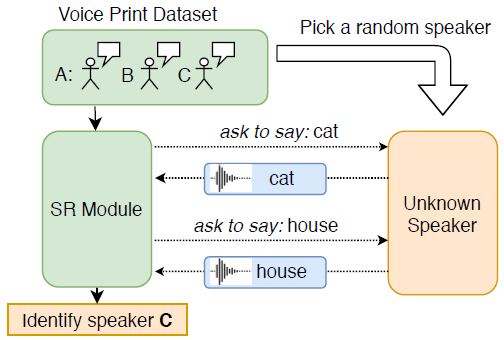
\includegraphics[width=.9\textwidth]{isr_game_large.png}
    \end{figure}

    \column{0.4\textwidth}
    Важные особенности статьи:
    \begin{enumerate}
        \item только идентификация
        \item фиксированный набор слов
        \item разные нейронные сети для запроса слов (\enquirer) и идентификации (\guesser)
    \end{enumerate}

    \end{columns}
\end{frame}

\begin{frame}{Архитектура \guesser}
\framesubtitle{Пытаемся угадать диктора}
    \begin{columns}
 
    \column{0.6\textwidth}
    \begin{figure}[bht]
    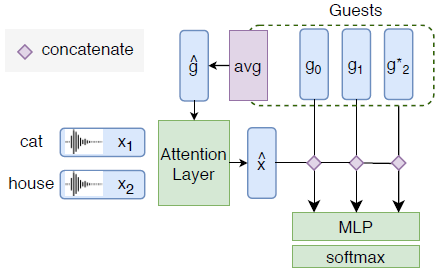
\includegraphics[width=.8\textwidth]{guesser.png}
    \end{figure}

    \column{0.4\textwidth}
    Входные данные:
    \begin{itemize}
        \item эмбеддинги дикторов\\
            $G = [g_1; g_2; \ldots g_K]$
        \item эмбеддинги слов\\
            $X = [x_1; x_2; \ldots x_T]$
    \end{itemize}
    Выходные данные:
    \begin{itemize}
        \item вероятности
            $\{P(g_i = g^*) \;|\; i=1..K\}$
    \end{itemize}
    \end{columns}

    \begin{block}{Обозначения}
    \begin{tabular}{l l}
        $K$ & количество гостей / дикторов\\
        $T$ & количество запрашиваемых слов
    \end{tabular}
    \end{block}
\end{frame}

\begin{frame}{Архитектура \enquirer}
\framesubtitle{Выбираем, какое слово мы спрашиваем у диктора}
    \begin{columns}

    \column{0.6\textwidth}
    \begin{figure}[bht]
    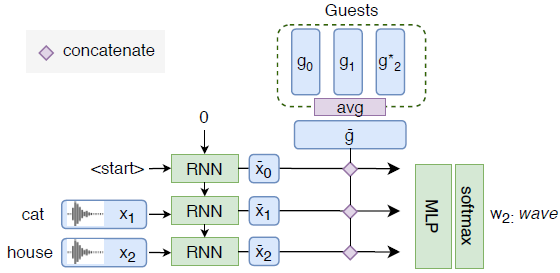
\includegraphics[width=.9\textwidth]{enquirer.png}
    % \caption{Архитектура блока Enquirer}
    \end{figure}

    \column{0.4\textwidth}
    Входные данные:
    \begin{itemize}
        \item среднее эмб. дикторов\\
            $\hat{g} = \frac{1}{K}{\sum_{i=1}^{K}{g_k}}$
        \item эмбеддинги слов\\
            $X = [x_1; x_2; \ldots; x_t]$
    \end{itemize}
    Выходные данные:
    \begin{itemize}
        \item вероятность выбрать каждое из слов
    \end{itemize}

    \end{columns}

    \begin{block}{Обозначения}
    \begin{tabular}{l l}
        $K$ & количество гостей / дикторов\\
        $T$ & количество запрашиваемых слов\\
        $t$ & количество запрошенных слов, $0 \leq t \leq T$
    \end{tabular}
    \end{block}
\end{frame}

\begin{frame}[t]{Обучение и тестирование \guesser{}}
    \framesubtitle{$K = 5$ дикторов  и $T = 3$ слова при обучении}
    \begin{columns}
        \centering
        \column{.5\textwidth}
        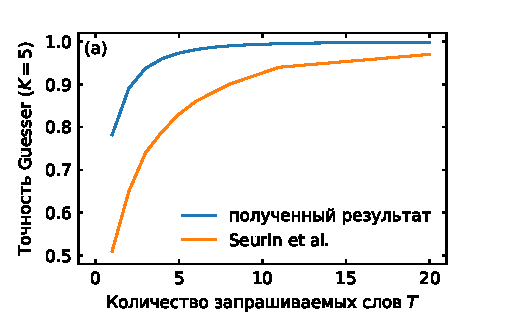
\includegraphics[scale=\imgscale]{../plots/word_sweep.pdf}
        \column{.5\textwidth}
        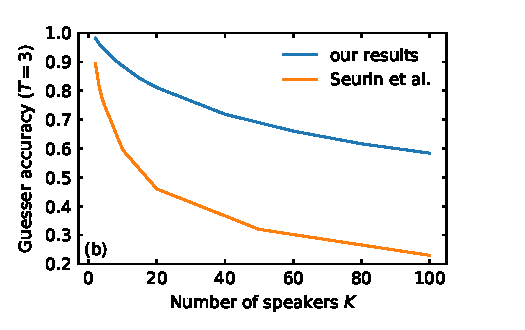
\includegraphics[scale=\imgscale]{../plots/guest_sweep.pdf}
    \end{columns}\vspace*{1em}

    Вероятно, главная причина расхождения результатов --- увеличение размерности
    эмбеддингов (512 вместо 128 в статье). Неизвестно, как и зачем в статье
    производилось понижение размерности.
\end{frame}

\begin{frame}[t]{Обучение и тестирование \enquirer{}}
    \framesubtitle{$K = 5$ дикторов  и $T = 3$ слова при обучении}
    \begin{columns}
        \centering
        \column{.5\textwidth}
        \only<1>{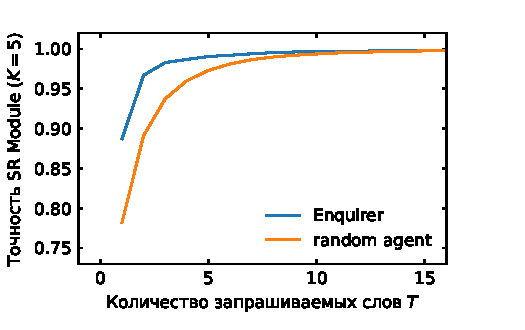
\includegraphics[scale=\imgscale]{../plots/word_sweep_enq.pdf}}
        \only<2>{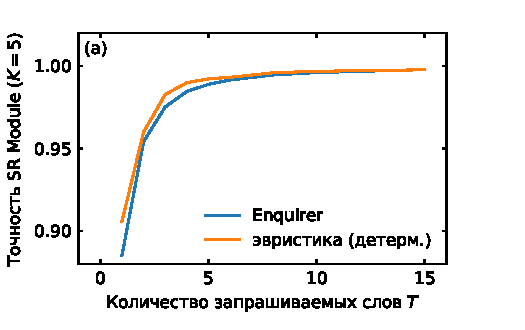
\includegraphics[scale=\imgscale]{../plots/word_sweep_heuristic.pdf}}
        \column{.5\textwidth}
        \only<1>{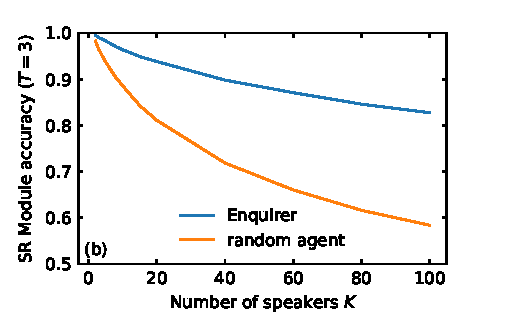
\includegraphics[scale=\imgscale]{../plots/guest_sweep_enq.pdf}}
        \only<2>{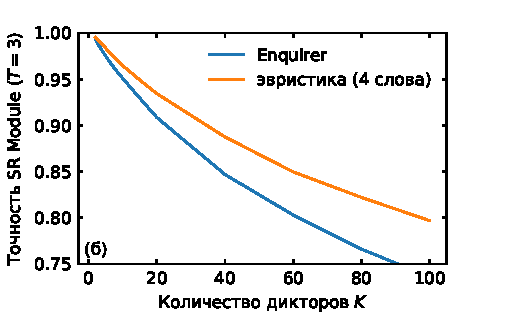
\includegraphics[scale=\imgscale]{../plots/guest_sweep_heuristic.pdf}}
    \end{columns}\vspace*{1em}
    Для обучения использовалась \textbf{PPO}. Выбор слова при обучении и
    тестировании проводился по-разному:
    \begin{itemize}
        \item \texttt{train} --- сэмплирование из распределения,
        \item \texttt{test} --- $\arg \max$ по не использованным ранее словам.
    \end{itemize}

    \only<2>{
        Эвристический агент не обращает внимание на контекст и (практически)
        всегда запрашивает одни и те же слова.
    }
\end{frame}

\begin{frame}{От идентификации к верификации}
    \framesubtitle{$T = 3$ слова}
    \begin{center}
    \only<1>{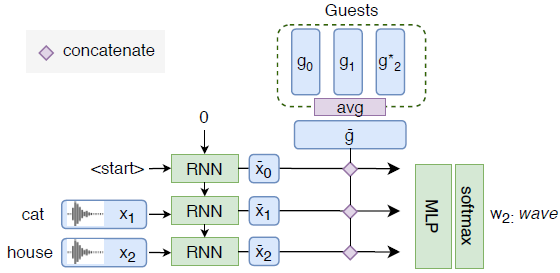
\includegraphics[scale=.6]{enquirer.png}}
    \only<2->{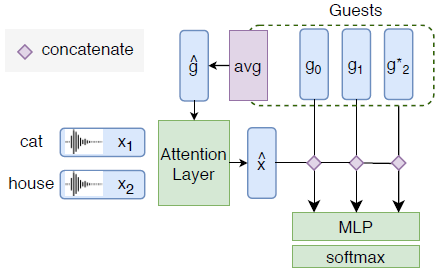
\includegraphics[scale=.6]{guesser.png}}
    \end{center}

    \begin{columns}
        \column{0.5\textwidth}
        \begin{itemize}
            \item<1-> \enquirer{}: не меняем ничего (даже веса)
            \item<2-> \guesser{}: меняем \texttt{softmax} на \texttt{sigmoid}
        \end{itemize}


        \column{0.5\textwidth}
        \onslide<3->{
        \begin{center}
            \begin{tabular}{c c}
                \toprule
                Выбор слов & Точность\\
                \midrule
                случайный & 0.895\\
                \enquirer{} & 0.933\\
                эвристика & 0.917\\
                \bottomrule
            \end{tabular}
        \end{center}
        }
        \end{columns}
\end{frame}

\begin{frame}{Обучение в более тяжелом режиме}
    \only<2>{
        \begin{table}[htb]
            \begin{tabular}{c c c}
                \toprule
                Выбор слов & Режим обучения & Точность\\
                \midrule
                случайный & \multirow{3}{4em}{$K = 5$\newline$T = 3$} & 0.937 \\
                \enquirer{} & & 0.982\\
                эвристика & & 0.984\\
                \midrule
                случайный & \multirow{3}{4em}{$K = 20$\\$T = 2$} & 0.951 \\
                \enquirer{} & & 0.989\\
                эвристика & & 0.988\\
                \bottomrule
            \end{tabular}
            \caption{Точность идентификации, $K = 5$ дикторов, $T = 3$
                     запрашиваемых слова}
        \end{table}
    }
    \only<1>{
        \begin{table}[htb]
            \begin{tabular}{c c c}
                \toprule
                Выбор слов & Режим обучения & Точность\\
                \midrule
                случайный & \multirow{3}{4em}{$T = 3$} & 0.895 \\
                \enquirer{} & & 0.933\\
                эвристика & & 0.917\\
                \midrule
                случайный & \multirow{3}{4em}{$T = 2$} & 0.913 \\
                \enquirer{} & & 0.947\\
                эвристика & & 0.945\\
                \bottomrule
            \end{tabular}
            \caption{Точность верификации, $T = 3$ запрашиваемых слова}
        \end{table}
    }
\end{frame}

\begin{frame}{Другие эксперименты}
    \begin{enumerate}
        \item \texttt{CodebookEnquirer} --- гибкая система выбора слов.
        \begin{itemize}
            \item Меняем последний слой \enquirer{}: теперь он выдает не вероятности
            выбрать то или иное слово из словаря, а эмбеддинг.
            \item Создаем \texttt{Codebook} --- набор эмбеддингов слов
            (усредняем по обучающей выборке).
            \item Для получения вероятностей считаем \texttt{softmax} с
            отрицательной температурой от расстояний между выходным эмбеддингом
            и эмбеддингами слов в \texttt{Codebook}.
            \item Работает (небольшое падение точности), даже если мы обучаем
            и тестируем модель на разных наборах слов.
        \end{itemize}

        \item Добавление шума
        \begin{itemize}
            \item Добавляем к аудиозаписям слов 6 видов шума из MUSAN\@.
            \item Не меняем тип шума в течение игры.
            \item Не помогает \enquirer{} опережать эвристику.
        \end{itemize}
    \end{enumerate}
\end{frame}

\begin{frame}{Выводы}
    \begin{itemize}
        \item Исследованный подход работает --- точность идентификации 
        существенно повышается при добавлении выбирающего слова
        агента.
        \item Модель можно сделать практически полезной: легко перейти от
        идентификации к верификации и от фиксированного набора слов к
        произвольному.
        \item В большинстве режимов (очень) простая эвристика оказывается не хуже
        нейросетевого агента для выбора слов (\enquirer{}).
    \end{itemize}
\end{frame}

% \begin{frame}[noframenumbering, plain]{}
% \end{frame}

\end{document}